\newpage
\section{Auswertung}
\label{sec:Auswertung}

\subsection{Messungen der Fourierkoeffizienten}
Der Vergleich der verschiedenen Spannungen erfolgt über die prozentuale Abweichung.

\subsubsection{Messung Rechtecksfunktion}
 Bei der Messung der Rechteckspannung ergeben sich die in Tab.1
 enthaltenen Werte. Zur Berechnung von $a_\text{n,theo} $ wurde
 Gleichung(\ref{eqn:rechteck}) verwendet.

 \begin{table}[h]
   \centering
   \label{rech}
   \begin{tabular}{ c c c c }
     \toprule
    $ \text{Oberschwingung n} $
    &$ a_\text{n,exp} \, \text{in [V]} $
    %&$ \text{\nu \, in  \, [Hz]} $
    &$ a_\text{n,theo} \,  \text{in  [V]} $
    &$ \text{Abweichung in} \, \si{\percent} $ \\

     \midrule
     1 &456   & 509.25 & 10.46 \\
     3 &148  & 169.76 & 12.82 \\
     5 & 84    & 101.86 & 17.53  \\
     7 & 54    &  72.76 & 25.78 \\
     9 & 43.2   &  56.59 & 23.66 \\
     11 & 37.6  &  46.59 &  18.79 \\
     13 & 32.0  &  39.18 & 18.31 \\
     15 & 30.4  & 33.95 & 10.46 \\
     17 & 26.4  & 29.96 & 11.88 \\
     \bottomrule
   \end{tabular}
   \caption{Werte der Rechteckspannung.}
 \end{table}

\subsubsection{Messung Dreiecksfunktion}
Die Werte sind in Tab.2 enthalten und werden für $a_\text{n,theo} $ mit Gleichung(\ref{eqn:dreieck})
errechnet.
  \begin{table}[h]
    \centering
    \label{tab:2}
    \begin{tabular}{ c c c c  }
      \toprule
     $ \text{Oberschwingung n} $
     &$ a_\text{n,exp} \, \text{in [V]} $
     %&$ \text{\nu \, \, in \, \, [Hz]} $
     &$ a_\text{n,theo} \, \text{in  [V]} $
     &$ \text{Abweichung in} \, \si{\percent} $\\

      \midrule
      1& 296.00    & 254.65 & 16.24\\
      3& 29.60  & 28.29 & 4.61\\
      5&  11.20 & 10.19 & 9.96\\
      7&  5.20 & 5.20 &0.00\\
      9&  3.44 & 3.14 &9.42\\
      11& 2.08 & 2.11& 1.17\\
      13& 1.52 & 1.52& 0.88\\
      15& 1.20 & 1.13& 6.03\\
      17& 0.96 & 0.88&8.95\\
      \bottomrule
    \end{tabular}
    \caption{Werte der Dreiecksspannung.}
  \end{table}
  \subsubsection{Messung Sägezahnfunktion}
  Für die Sägezahnspannung wird $a_\text{n,theo} $ mit Gleichung(\ref{eqn:saege})
  errechnet. Die Werte sind in Tab.3 enthalten.
  \begin{table}[h]
    \centering
    \label{tab:3}
    \begin{tabular}{ c c c c  }
      \toprule
     $ \text{Oberschwingung n} $
     &$ a_\text{n,exp} \, \text{in [V]} $
     %&$ \text{\nu \, \, in \, \, [Hz]} $
     &$ a_\text{n,theo} \, \text{in  [V]} $
     &$ \text{Abweichung in} \, \si{\percent} $\\

      \midrule
      1&236  & 254.65& 7.32 \\
      2&118  & 127.32& 7.32\\
      3& 78  &  84.88& 8.10\\
      4& 56.8&  63.66& 10.78\\
      5& 44  &  50.93& 13.61\\
      6& 36  &  42.44& 15.17\\
      7& 28.8&  36.38& 20.83\\
      8& 24.8&  31.83& 22.09\\
      9& 21.6&  28.39& 23.66\\

      \bottomrule
    \end{tabular}
    \caption{Werte der Sägezahnspannung.}
  \end{table}

\subsection{Fourier-Synthese}
Mit Hilfe der Gleichungen (\ref{eqn:rechteck}),(\ref{eqn:dreieck}) und (\ref{eqn:saege})
werden die bereits vorher zerlegten Funktionen aus verschiedenen Oberschwingungen so zusammengelegt,
dass sie der Form der Spannungen entsprechen. Im folgenden werden die Ergebnisse in Form von Bildern hinzugefügt.

\subsubsection{Rechteckspannung}
Die verwendeten Spannungen um die gesuchten Oberschwingungen zu generieren ist Tab.4 zu entnehmen.
Mit diesen ergibt sich eine Rechteckspannung wie sie in Abb.(\ref{fig:recht}) zu sehen ist.
\begin{table}[h]
  \centering
  \label{tab:4}
  \begin{tabular}{ c c c c c c  }
    \toprule
   $ \text{Oberschwingung n} $ & 1 & 3 & 5 & 7 & 9 \\
    \midrule
   $\increment{U} \,\text{in\,[V]}$ &90 & 30 &18 &12.9 & 10 \\
    \bottomrule
  \end{tabular}
  \caption{Spannungen für Rechtecksspannung.}
\end{table}
\begin{figure}[H]
  \centering
  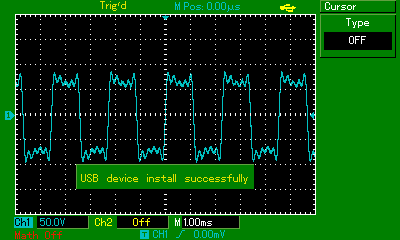
\includegraphics{content/images/rechteck.png}
  \caption{Rechtecksspannung.}
  \label{fig:recht}
\end{figure}
\subsubsection{Dreiecksspannung}
Analog zur Rechteckspannung wird die Dreiecksspannung erstellt. Die Spannungen
sind Tab.5 zu entnehmen und die Form ist in Abb.(\ref{fig:dreie}) zu sehen.
\begin{table}[h]
  \centering
  \label{tab:5}
  \begin{tabular}{ c c c c c c }
    \toprule
   $ \text{Oberschwingung n} $ & 1 & 3 & 5 & 7 & 9 \\
    \midrule
   $\increment{U}\, \text{in\,[V]}$ &90 & 10 &3.6 &1.84 & 1.11 \\
    \bottomrule
  \end{tabular}
  \caption{Spannungen für Dreiecksspannung.}
\end{table}
\begin{figure}[H]
  \centering
  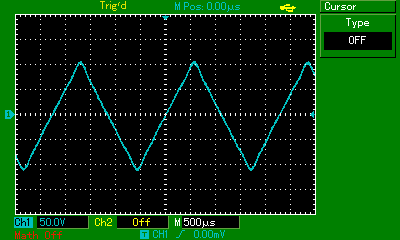
\includegraphics{content/images/dreieck.png}
  \caption{Dreiecksspannung.}
  \label{fig:dreie}
\end{figure}
\subsubsection{Sägezahnspannung}
Die für die Sägezahnspannung  in Abb.(\ref{fig:saeg}) verwendeten Spannung sind Tab.6 zu entnehmen.

\begin{table}[h]
  \centering
  \label{tab:6}
  \begin{tabular}{ c c c c c c c c c c c }
    \toprule
   $ \text{Oberschwingung n} $ & 1 &2 &  3 & 4& 5 &6& 7&8 & 9 & 10\\
    \midrule
   $\increment{U} \, \text{in\,[V]}$ &90& 45 & 30 & 22.5 &18 & 15 & 12.9 & 11.25 & 10 & 9 \\
    \bottomrule
  \end{tabular}
  \caption{Spannungen für Sägezahnspannung.}
\end{table}
\begin{figure}[H]
  \centering
  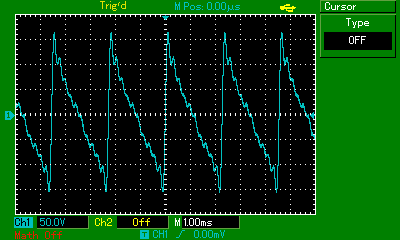
\includegraphics{content/images/saegezahn.png}
  \caption{Sägezahnspannung.}
  \label{fig:saeg}
\end{figure}
